%! Licence = CC BY-NC-SA 4.0

%! Author = gianfluetsch
%! Date = 22. Jan 2022
%! Project = icth_summary

\section{Quellencodierung}

\subsection{Kompression/ Komprimierung}

\subsubsection{Nachprüfung HS2020}
\begin{center}
    \centering
    \begin{tabular}{l | l}
        \bfseries{Zeichen} & \bfseries{Wahrscheinlichkeit p(x)}\\ \hline
        a & 0.4\\ 
        b & 0.3\\
        c & 0.2\\
        d & 0.1\\
    \end{tabular}
\end{center}

\paragraph{Entropie der Quelle}\mbox{}\\
$I(x) = log_{2}(\frac{1}{p(x)})$\\
$H(x) = p(x)*I(x)$\\
$H(x) = 0.4*log_2\frac{1}{0.4}+0.3*log_2\frac{1}{0.3}+0.2*log_2\frac{1}{0.2}+0.1*log_2\frac{1}{0.1}=1.846$

\paragraph{Redundanz der Quelle}\mbox{}\\
$H_0 = log_2(N) = log_2(4) = 2 \rightarrow$ (N = Anzahl Zeichen)\\
$R_0 = H_0 - H(x) = 2-1.846=0.153$

\paragraph{Redundanz des Codes mit Codierung}
\begin{center}
    \centering
    \begin{tabular}{l | l}
        \bfseries{Zeichen} & \bfseries{Codierung}\\ \hline
        a & 001\\ 
        b & 010\\
        c & 011\\
        d & 100\\
    \end{tabular}
\end{center}
$L = p*L \rightarrow p_1*L_1+p_2*L_2...$\\
$R_c = L - H(x) \rightarrow$ L=Anzahl Bits (3)\\
$3-1.846=1.154$

\paragraph{Huffman-Code erstellen (Codierung)}\mbox{}\\
\begin{center}
    \centering
    \begin{tabular}{l | l}
        \bfseries{Zeichen} & \bfseries{Codierung}\\ \hline
        a & 1\\ 
        b & 01\\
        c & 001\\
        d & 000\\
    \end{tabular}
\end{center}

\paragraph{Redundanz Huffman-Code}\mbox{}\\
$L=0.4*1+0.3*2+0.2*3+0.1*3=1.9$\\
$R_c = L-H(x) = 1.9-1.846=0.054$

\paragraph{Codieren sie ''aaabbacd'' mit Huffman-Code}\mbox{}\\
$a\_a\_a\_\_b\_\_b\_\_\_a\_\_c\_\_d$\\
$1\_1\_1\_|\_01\_01\_|\_1\_001\_000 \rightarrow 14 Bits$

\paragraph{Lauflängencodierung der Bitfolge}\mbox{}\\
Orginale Bitfolge: $11101011001000 \rightarrow |w_c| = 14 bit$\\
Code: $3$ $1$ $1$ $1$ $2$ $2$ $1$ $3 \rightarrow$ mit 2 Bits kann Code codiert werden\\
Bitfolge komprimiert: $11$ $01$ $01$ $01$ $10$ $10$ $01$ $11$\\
$\rightarrow |w_c| = 16 bit$

\paragraph{Kompression im Vergleich}\mbox{}\\
Ursprünglich: $8\_Zeichen * 3\_Bit = 24 Bit$\\
Huffman: $14 Bit$\\
$\rightarrow 14Bit/24Bit=0.5833=58\%$

\paragraph{Min. theoretische Redundanz Huffman}\mbox{}\\
% TODO: ???

\paragraph{Wann wird das erreicht?}\mbox{}\\
% TODO: ???

\subsubsection{Prüfung FS2017}
\begin{center}
    \centering
    \begin{tabular}{l | l}
        \bfseries{Zeichen} & \bfseries{Wahrscheinlichkeit p(x)}\\ \hline
        a & 0.5\\ 
        b & 0.25\\
        c & 0.1\\
        d & 0.1\\
        e & 0.05
    \end{tabular}
\end{center}

\paragraph{Entscheidungsgehalt $H_0$ des Codes}\mbox{}\\
$H_0=log_2(N) \rightarrow$ N = Anzahl Zeichen\\
$H_0=log_2(5)=2.322$

\paragraph{Redundanz der Quelle}\mbox{}\\
$H(x) = p(x)*I(x)$\\
$I(x) = log_2(\frac{1}{p(x)})$\\
$H(x) = 0.5*1+0.25*2+0.1*3.322+0.1*3.322+0.05*4.322=1.88$
$R_0 = H_0 - H(x) = 2.322-1.88=0.44$

\paragraph{Mittlere Codewortlänge \&Redundanz des Codes}\mbox{}\\
\begin{center}
    \centering
    \begin{tabular}{p{1cm} | p{1.5cm} | p{1.5cm} | p{1.25cm}}
        \bfseries{Zeichen} & \bfseries{Codierung} & \bfseries{Länge (L)} & \bfseries{Mittlere Länge}\\ \hline
        a & 1 & 1 & 0.5\\ 
        b & 01 & 2 & 0.5\\
        c & 0100 & 4 & 0.4\\
        d & 1000 & 4 & 0.4\\
        e & 11000 & 4 & 0.25
    \end{tabular}
\end{center}
$L = p*L \rightarrow p_1*L_1+p_2*L_2...$\\
$L=0.5+0.5+0.4+0.4+0.25=2.05$\\
$R_c = L - H(x)$\\
$2.05-1.88=0.17$

\paragraph{Optimierung Codierung nach Huffman}\mbox{}\\
Wie viel Prozent kann Redundanz in Code mit Huffman gegenüber ursprünglichem Code reduziert werden?\\
\begin{center}
    \vspace{-8pt}
    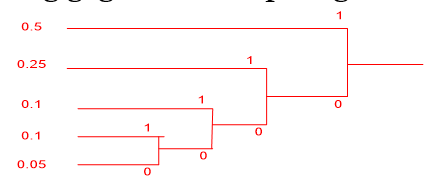
\includegraphics[width=.5\linewidth]{./01-quellencodierung/optimierung_codierung}
    \vspace{-8pt}
\end{center}

\begin{center}
    \centering
    \begin{tabular}{l | l}
        \bfseries{Zeichen} & \bfseries{Huffman}\\ \hline
        a & 1\\ 
        b & 01\\
        c & 001\\
        d & 0001\\
        e & 0000\\
    \end{tabular}
\end{center}

Daraus folgt für die Redundanz nach Huffman = 0.02. 
Das sind 11.8\% und entspricht einer Redundanzreduktion um 88.2\%.

\subsubsection{Prüfung HS2016}
Der Informationsgehalt einer Bildvorlage soll über einen Binärkanal mit der Kanalkapaziät von 40 kBit/sec übertragen werden. Dabei wird das Bild durch Abtastung in 105 Bildpunkte zerlegt. Ein Bild-punkt kann in 8 Helligkeitswerte H zerlegt werden.

\paragraph{Welche Übertragungszeit ergibt sich, wenn alle Helligkeitswerte gleich codiert werden?}\mbox{}\\
$L_D 8=3$ Bit pro Bildpunkt\\
$\rightarrow TÜ = 3*10^5:40kBit/sec=7.5sec$\\

Nähere Untersuchungen der Helligkeitswerte ergeben für die Helligkeitswerte H1 bis H8 folgende Ver-teilung ihrer Auftrittswahrscheinlichkeit:
\begin{center}
    \centering
    \begin{tabular}{l | l}
        \bfseries{H} & \bfseries{P}\\ \hline
        H1 & 0.4\\ 
        H2 & 0.35\\
        H7 & 0.1\\
        H4 & 0.0625\\
        H3 & 0.035\\
        H5 & 0.03225\\
        H6 & 0.01425\\
        H8 & 0.006
    \end{tabular}
\end{center}

\paragraph{Um wie viel Prozent können sie die Übertragungsgeschwindigkeit eines Bildes verkürzen, wenn sie die erfassten Bildpunkte vor dem Versenden nach Huffmann codieren?}\mbox{}\\
\begin{center}
    \centering
    \begin{tabular}{p{1cm} | p{1cm} | p{1cm} | p{1cm} | p{1cm}}
        \bfseries{H} & \bfseries{P} & \bfseries{Möglicher Code} & \bfseries{Anzahl Bits} & \bfseries{Länge}\\ \hline
        H1 & 0.4 & 0 & 1 & 0.4\\ 
        H2 & 0.35 & 10 & 2 & 0.7\\
        H7 & 0.1 & 110 & 3 & 0.3\\
        H4 & 0.0625 & 1110 & 4 & 0.25\\
        H3 & 0.035 & 11110 & 5 & 0.175\\
        H5 & 0.03225 & 111110 & 6 & 0.1935\\
        H6 & 0.01425 & 1111110 & 7 & 0.09975\\
        H8 & 0.006 & 1111111 & 7 & 0.042\\
        Total & & & & 2.16025
    \end{tabular}
\end{center}

$TÜ=2.16*10^5:40kBit/sec = 5.4sec$\\
$7.5=100\%$\\
$5.4 = 5.4/7.5*100\% = 72\%$\\
Daraus folgt eine Verbesserung um 28\%.

\paragraph{Für den Kanal konnte die folgende Kanalmatrix P(Y|X) ermittelt werden.}\mbox{}\\
$P(X|Y) = \begin{matrix}
    0.9 & 0.1\\
    0.1 & 0.9\\
\end{matrix}$

Wie lange dauert es dann mindestens, bis alle Daten fehlerfrei übertragen sind? Gehen Sie davon aus das „0“ und  „1“ gleich wahrscheinlich sind. \\
$TÜ = 2.16*10^5:(1000*40Bit)=5.4sec$

\subsection{Huffman}
\subsubsection{Prüfung HS2009}
Gegeben sind die folgenden Zeichen a, b, c, d mit den Auftrittswahrscheinlichkeiten 
P{a} = 0.5, P{b}= 0.25, P{c} = 0.125, P{d}= 0.125\\

Zeigen Sie, dass eine nach Huffmann codierte Quellencodierung einen Redundanzfreien 
Code ergibt.
\begin{center}
    \vspace{-8pt}
    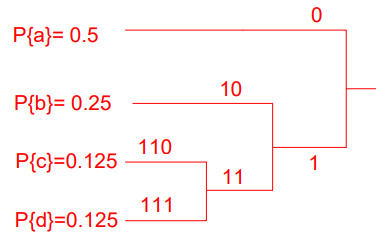
\includegraphics[width=.5\linewidth]{./01-quellencodierung/hs2009}
    \vspace{-8pt}
\end{center}

$H(X) = 0.5*log_2(\frac{1}{0.5})+0.25*log_2(\frac{1}{0.25})+0.125*log_2(\frac{1}{0.125})=1.75$\\
$L=0.5*1+0.25*2+0.125*3+0.125*3=1.75$\\
$R_c=L-H(x)=0$

\subsubsection{Prüfung FS2009}
Codieren Sie die nachfolgenden Zeichen mit der Huffmancodierung\\
\textit{ABRAKADABRA}\\

\paragraph{Auftrittswahrscheinlichkeit pro Zeichen}\mbox{}\\
$\frac{Häufigkeitsverteilung Zeichen}{Anzahl Symbole}$

\begin{center}
    \centering
    \begin{tabular}{p{1.9cm} | p{0.5cm} | p{0.5cm} | p{0.5cm} | p{0.5cm} | p{0.5cm} }
        \bfseries{Symbol} & \bfseries{A} & \bfseries{B} & \bfseries{R} & \bfseries{K} & \bfseries{D}\\ \hline
        Häufigkeitsvert. & 5 & 2 & 2 & 1 & 1\\ 
        p(Symbol) & 0.45 & 0.18 & 0.18 & 0.09 & 0.09
    \end{tabular}
\end{center}

\paragraph{Informationsgehalt pro Zeichen}\mbox{}\\
$I(x)=log_2(\frac{1}{p(x)}) \rightarrow [I(x)]=bit$

\begin{center}
    \centering
    \begin{tabular}{p{1.9cm} | p{0.5cm} | p{0.5cm} | p{0.5cm} | p{0.5cm} | p{0.5cm} }
        \bfseries{Symbol} & \bfseries{A} & \bfseries{B} & \bfseries{R} & \bfseries{K} & \bfseries{D}\\ \hline
        Häufigkeitsvert. & 5 & 2 & 2 & 1 & 1\\ 
        I(x) & 1.37 & 2.45 & 2.45 & 3.45 & 3.45
    \end{tabular}
\end{center}

\paragraph{Huffmancodierung}\mbox{}\\
% TODO:

\subsection{Diskrete Quelle mit Gedächtnis}
\subsubsection{Prüfung FS2009}
Ein Code hat die durch das angegebene Markoffdiagramm gegeben inneren Abhängigkeiten.\\

Ergänzen Sie die fehlenden Wahrscheinlichkeitswerte im Diagramm.
\begin{center}
    \vspace{-8pt}
    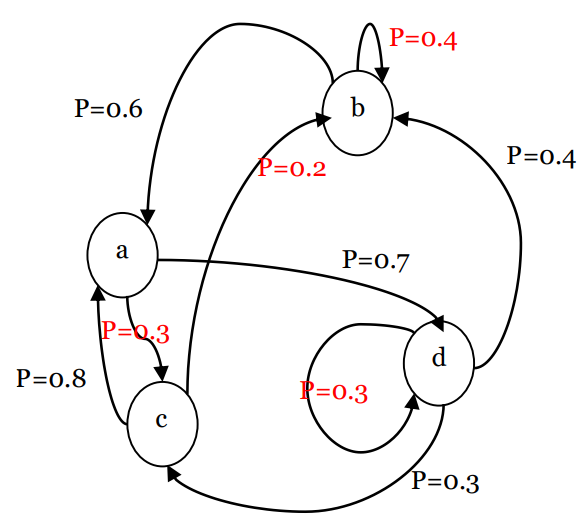
\includegraphics[width=.5\linewidth]{./01-quellencodierung/hs2009_1}
    \vspace{-8pt}
\end{center}

Bestimmen Sie die Entropie des Codes H(X) sowie die Verbundentropie H(X|Y). Um wieviel Prozent kann die Redundanz gesenkt werden, wenn die inneren Abhängigkeiten berücksichtigt werden?\\
% TODO

\subsubsection{Prüfung HS2009}
Sie untersuchen eine diskrete Quelle mit Gedächtnis. Die Quelle hat den folgenden Zeichensatz: A, B, C\\
Die bedingte Wahrscheinlichkeit ist gegeben:\\
$\begin{matrix}
    P(A|A) & P(B|A) & P(C|A)\\
    P(A|B) & P(B|B) & P(C|B)\\
    P(A|C) & P(B|C) & P(C|C)
\end{matrix} = \begin{matrix}
    0 & 1/5 & 8/10\\
    1/10 & 1/2 & 2/5\\
    9/20 & 1/2 & 1/20
\end{matrix}$

Zeichnen Sie das Markoff-Diagramm.
\begin{center}
    \vspace{-8pt}
    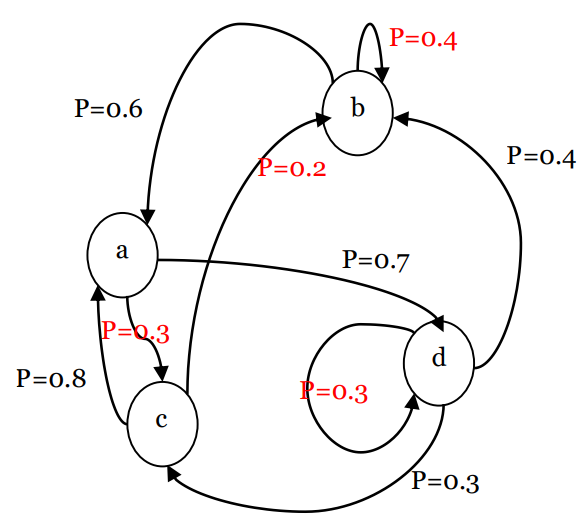
\includegraphics[width=.5\linewidth]{./01-quellencodierung/hs2009_1}
    \vspace{-8pt}
\end{center}

\columnbreak

\subsection{Lempel-Ziv}
\subsubsection{Prüfung FS2009}
Codieren Sie die nachfolgende Bitfolge mit dem Lempel-Ziv 77 Verfahren:\\
$01101110101010001101110$
\begin{center}
    \vspace{-8pt}
    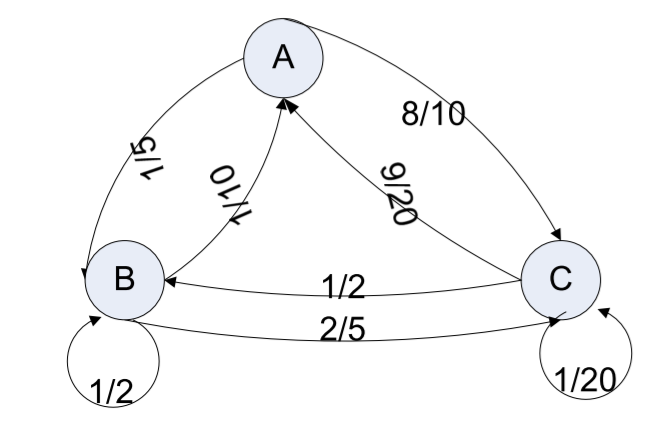
\includegraphics[width=.8\linewidth]{./01-quellencodierung/hs2009_2}
    \vspace{-8pt}
\end{center}

Bestimmen Sie die Auftrittswahrscheinlichkeiten der Zeichen\\
$P(A)=iP(B)+1/10+P(C)*9/20$\\
$P(B)=P(A)*1/5+P(B)*1/2+P(C)*1/2$\\
$P(C)=P(A)*8/10+P(B)*2/5+P(C)*1/20$\\
$1=P(A)+P(B)+P(C)$\\

$P(A)=\frac{55}{269}=0.20$\\
$P(B)=\frac{118}{269}=0.43$\\
$P(C)=\frac{96}{269}=0.34$






